\documentclass{standalone}
\usepackage{tikz}
\usetikzlibrary{shapes,arrows.meta}
\begin{document}
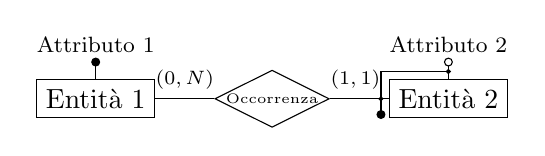
\begin{tikzpicture}
    \draw

    %%* Attributi:
    %%  node[draw, circle, inner sep=1pt, fill=black]{}node[right]{\footnotesize A}
    %%? Distanza orizzontale: E -(0.25,0.x)- A
    %%? Distanza verticale: E -(0,x * 0.22)- A

    %%* Cardinalità:
    %%  node[below right]{\scriptsize $(0,N)$}
    %%  node[above right]{\scriptsize $(0,N)$}
    %%  node[midway, above]{\scriptsize $(0,N)$}

    %%* Relazione:
    %%  node[draw, diamond, shape aspect=2, inner sep=3pt, anchor=90](r1){}
    %%  node[draw, diamond, shape aspect=2, inner sep=0.2pt, anchor=180](r2){R2}

    %%* Entità:
    %%  node[draw, rectangle, anchor=90](e1){}
    %%? Distanza verticale: E -(0.3)- R -(0.3) E
    %%? Distanza orizzontale: E -(0.75)- R -(0.75)- E
    
    (0,0)node[draw, rectangle, anchor=90](e1){Entità 1}
    (e1.90)--++(0,0.22)node[draw, circle, inner sep=1pt, fill=black]{}node[above]{\footnotesize Attributo 1}
    (e1.0)--++(0.75,0)node[draw, diamond, shape aspect=2, inner sep=0.2pt, anchor=180](r1){\tiny Occorrenza}node[midway, above]{\scriptsize $(0,N)$}
    (r1.0)--++(0.65,0)node[draw, circle, inner sep=0.5pt, fill=black](a){}node[midway, above]{\scriptsize $(1,1)$}--++(0.1,0)node[draw, rectangle, anchor=180](e1){Entità 2}
    (e1.90)--++(0,0.1)node[draw, circle, inner sep=0.5pt, fill=black](b){}--++(0,0.12)node[draw, circle, inner sep=1pt, fill=white]{}node[above]{\footnotesize Attributo 2}
    (a)--++(0,-0.2)node[draw, circle, inner sep=1pt, fill=black]{}|-(b)

    ;
\end{tikzpicture}
\end{document}